\newacronym{owl}{OWL}{Web Ontology Language}
\newacronym{dcmi}{DCMI}{Dublin Core Metadata Initiative}
\newacronym{rdfs}{RDFS}{Resource Description Framework Schema}
\newacronym{rdf}{RDF}{Resource Description Framework}
\newacronym{dc}{DC}{Dublin Core}
\newacronym{skos}{SKOS}{Simple Knowledge Organization System}
\newacronym{uri}{URI}{Uniform Resource Identifier}
\newacronym{w3c}{W3C}{World Wide Web Consortium}

\section{Embedded Context}\label{sec:embedded_context}
In this section we describe another approach of generating Context descriptions based on semantic metadata.
For that, we used \hyperref[sec:OWL_annotation_properties]{Annotation~Properties} which were defined as part of \hyperref[sec:OWL_annotation_properties]{\gls{owl}\footnote{\url{https://www.w3.org/OWL/} accessed 2018/18/12}}. To maximise interoperability with existing libraries for ontology processing and manipulation we made use of the \hyperref[sec:dublin_core_metadata_vocabulary]{Dublin~Core~Metadata~Set}, a standard vocabulary designed to annotate resources with simple, textual information. A prerequisite for Context generation is the presence of such metadata information.
However, as none of our ontologies contained such metadata, we had to add them manually. 

This section starts by introducing annotation properties which are defined as part of \gls{owl}. We used annotations to encode the Context descriptions. Next, an overview of the \hyperref[sec:dublin_core_metadata_vocabulary]{Dublin~Core~Metadata~Set} is given as some parts were used for the definition of Context properties. Then, in the remainder of this section our \hyperref[sec:enrichment_metaData_approach]{Metadata~based~Approach} is discussed.

\subsection{\gls{owl} Annotation Properties}\label{sec:OWL_annotation_properties}
Annotation properties first defined by \gls{owl}~1\footnote{\url{https://www.w3.org/TR/owl-ref/\#Annotations} accessed 2018/20/12} and then extended by \gls{owl}~2\footnote{\url{https://www.w3.org/TR/owl2-syntax/\#Annotation_Properties} accessed 2018/20/12} are used to enhance concepts, properties, individuals and ontology headers with meta data such as labels, comments, creation date and so forth. This information does not alter the semantics of the ontology in any way, it is merely intended for documentation purposes and therefore ignored by reasoning engines. 

Besides the built-in annotation properties \gls{owl}~1 also offers the ability to create user-defined annotation properties. An example of using \emph{owl:AnnotationProperty} to declare a user-defined annotation property is given in~\hyperref[lst:user_defined_annotation_property]{Listing~\ref*{lst:user_defined_annotation_property}}. In this example, the \gls{owl}~Class \emph{Lens} is annotated with the custom annotation property \emph{dc:date} which is defined by the \hyperref[sec:dublin_core_metadata_vocabulary]{Dublin~Core~Metadata~Set} discussed in the next section. 
\begin{lstlisting}[frame=single,caption=Declaration of user-defined annotation property in \gls{owl}~1,label=lst:user_defined_annotation_property]
	<rdf:RDF
		xmlns:rdf="http://www.w3.org/1999/02/22-rdf-syntax-ns#"
		xmlns:dc="http://www.purl.org/metadata/dublin-core#"
		xmlns:owl="http://www.w3.org/2002/07/owl#">
		
		<owl:AnnotationProperty 
			rdf:about="http://purl.org/metadata/dublin-core#date"/>
		
		<owl:Class rdf:about="http://www.photo.org/camera#Lens"
			<dc:date rdf:datatype="http://www.w3.org/2001/XMLSchema#date">
				2018-12-20
			</dc:date>
		</owl:Class>
		
	</rdf>
\end{lstlisting}

\subsection{Ontology Metadata Standards}\label{sec:ontology_metadata_standards}
Over the years ontologies were used in many contexts, including general-purpose as well as highly specialised ones. Obviously, what separates good ontologies from poor ones is how well they are documented~\cite{daquin2012}. Studies~\cite{dutta2017} analysed various approaches of embedding metadata in ontologies. The outcome was that there is no standard way to describe and document ontologies, albeit a few vocabularies that describe semantic metadata exist. Two of the most common vocabularies are briefly described next.

\paragraph{Dublin Core Metadata Set}\label{sec:dublin_core_metadata_vocabulary} Being one of the most prominent vocabulary in describing semantic metadata, published and maintained by the \gls{dcmi}, it originally contained 15 metadata terms\footnote{\url{http://www.dublincore.org/documents/dces/} accessed 2018/05/20},  designed to annotate resources with simple, textual information. Since its first launch, the project have gained popularity, including more than 127 terms\footnote{\url{http://www.dublincore.org/documents/dcmi-terms/} accessed 2018/05/20}. The initial set of terms is listed in~\hyperref[app:dc_terms]{Appendix~\ref*{app:dc_terms}}. 

To maximise interoperability in heterogeneous environments, an \gls{rdf}-Schema with \gls{dcmi}-Metadata\footnote{\url{http://dublincore.org/schemas/rdfs/} accessed 2018/05/20} elements was created, in which each entity is identified by a \gls{uri} starting with the prefix \emph{http://purl.org}. A broader discussion on the use of metadata in general is given in~\cite{nilsson2010}.  

\paragraph{\gls{skos}}
The \gls{skos} Core Vocabulary \cite{skos2005} defines a set of \gls{rdf} properties and \gls{rdfs} classes
used to express the content and structure of a concept scheme, which describes sets of concepts with optionally linked concepts. The vocabulary is standardised by the \gls{w3c}\footnote{\url{https://www.w3.org/TR/skos-reference/} accessed 2018/05/20}. Relevant terms are listed in~\hyperref[app:skos_terms]{Appendix~\ref*{app:skos_terms}}.
	
There is some overlap between \gls{dc} and \gls{skos}. For example, the terms \textit{dc:subject} and \textit{skos:subject} describe similar characteristics of an entity. However, in some scenarios the range of skos:subject is limited to resources of type skos:concept compared to the unrestricted range of dc:subject. 


\subsection{Metadata based Approach}\label{sec:enrichment_metaData_approach}
Given the high number on ontology metadata formats from above, \hyperref[alg:embedded_enrichment]{Algorithm~\ref*{alg:embedded_enrichment}} shows the pseudocode to create concept descriptions extracted from embedded metadata. In addition to the notation used in the previous section we define $\Phi(C) \coloneqq \{m_1, m_2, \ldots, m_i \}$ where $m_i$ is the $i'th$ metadata element embedded in concept $C$ and $T$ is the description of some metadata element.

\begin{algorithm}
	\caption{Context Enrichment based on embedded metadata}\label{alg:embedded_enrichment}
	\begin{algorithmic}[1]
		\Procedure{Generate Description}{}\newline
			\textbf{Input:} A concept $C$ with embedded metadata $\{m_1, m_2, \ldots, m_i \}$\newline
			\textbf{Output:} A description $T$ of $C's$ metadata elements\newline
			\State{$T=\{\}$}
			\For {$ m_k \in \Phi(C) $}
				\State $T=T$ $\cup$ $m_k$
			\EndFor
		\EndProcedure
	\end{algorithmic}
\end{algorithm}

While the actual enrichment is straightforward, it collects all descriptions for a determined concept, the details of extracting the metadata from annotation properties is omitted here because it highly depends on the chosen metadata encoding.
As we decided to encode the metadata in annotation properties, the extraction process works by selecting the related annotation properties for a specified concept. 

To illustrate the concept of the Context generation algorithm a simple example of an \gls{owl}~Class enriched with metadata is shown in~\hyperref[lst:metadata_based_rdf_example]{Listing~\ref*{lst:metadata_based_rdf_example}}.
For that, the algorithm generates $T=\{$ \emph{"Greenhouse gas is one of several gases, especially carbon dioxide, that prevent heat from the earth escaping into space, causing the greenhouse effect. Greenhouse gases from human activities are the most significant driver of observed climate change since the mid-20th century.", "greenhouse gas"} $\}$. 
\hyperref[fig:metadata_rdf_example_questionaire]{Figure~\ref*{fig:metadata_rdf_example_questionaire}} depicts the questionnaire presented to crowd workers for the example from above. The text was constructed from the description defined by the Dublin~Core~Metadata~Set and the label defined by \gls{rdfs}\footnote{\url{https://www.w3.org/TR/rdf-schema/} accessed 2018/12/30}. 

\begin{lstlisting}[frame=single,breaklines=true,postbreak=\mbox{\textcolor{black}{$\hookrightarrow$}\space},caption=An \gls{owl} Class enriched with metadata,label=lst:metadata_based_rdf_example]
	<rdf:RDF
		xmlns:rdf="http://www.w3.org/1999/02/22-rdf-syntax-ns#"
		xmlns:rdfs="http://www.w3.org/2000/01/rdf-schema#"
		xmlns:dc="http://www.purl.org/metadata/dublin-core#"
		xmlns:owl="http://www.w3.org/2002/07/owl#">
		
		<owl:Class rdf:about="http://www.climatechange.org/greenhouse_gas"
			<dc:description>
				Greenhouse gas is one of several gases, especially carbon dioxide, that prevent heat from the earth escaping into space, causing the greenhouse effect. Greenhouse gases from human activities are the most significant driver of observed climate change since the mid-20th century.
			</dc:description>
			<rdfs:label>
				greenhouse gas
			</rdfs:label>
		</owl:Class>
		
	</rdf>
\end{lstlisting}

\begin{figure}
	 \centering
	 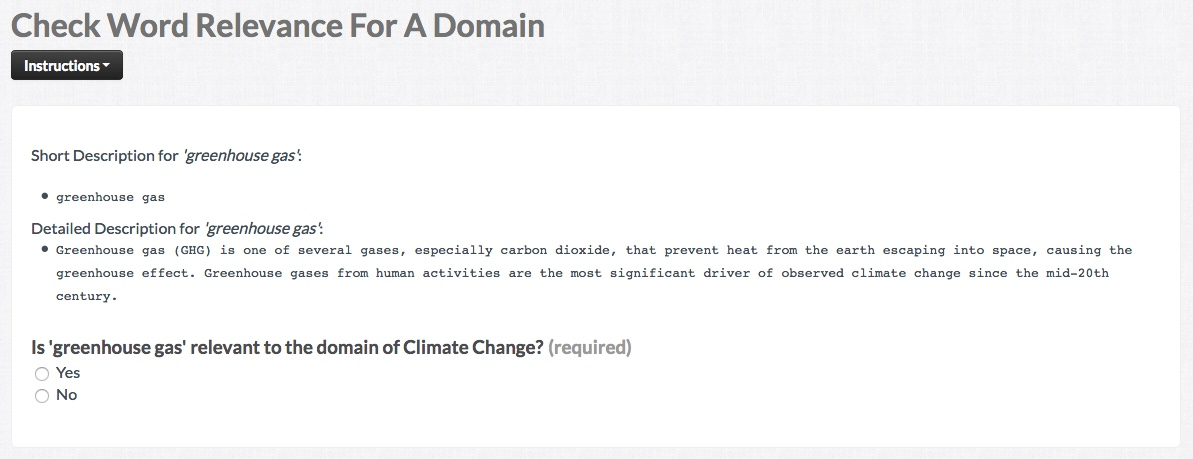
\includegraphics[width=\textwidth]{screenshots/questionaire_metadata_example}
	 \caption{Questionnaire presented to crowd workers for the \gls{owl} Class example}\label{fig:metadata_rdf_example_questionaire}
\end{figure}
